\documentclass[conference]{IEEEtran}
\usepackage{cite}
\usepackage{amsmath,amssymb,amsfonts}
\usepackage{algorithmic}
\usepackage{graphicx}
\usepackage{textcomp}
\usepackage{xcolor}
\def\BibTeX{{\rm B\kern-.05em{\sc i\kern-.025em b}\kern-.08em
    T\kern-.1667em\lower.7ex\hbox{E}\kern-.125emX}}
\begin{document}

\makeatletter
\newcommand{\newlineauthors}{%
  \end{@IEEEauthorhalign}\hfill\mbox{}\par
  \mbox{}\hfill\begin{@IEEEauthorhalign}
}
\makeatother

\title{Portable Visible Spectrophotometer for Glucose Microdroplet Measurements in Digital Microfluidics System}

\author{\IEEEauthorblockN{
    Alzana Armaniar Farhani\IEEEauthorrefmark{1},
    Balkan Khilmi Assakandari\IEEEauthorrefmark{2},
    Anindhita Nayazirly\IEEEauthorrefmark{3}, \\
    Akhmadi Surawijaya\IEEEauthorrefmark{4},
    Muhammad Ogin Hasanuddin\IEEEauthorrefmark{5}}
\IEEEauthorblockA{\textit{Department of Electrical Engineering} \\
\textit{School of Electrical Engineering and Informatics} \\
\textit{Institut Teknologi Bandung}\\
Bandung, Indonesia \\
\IEEEauthorrefmark{1}farhanialzana@gmail.com,
\IEEEauthorrefmark{2}balkankhilmi@gmail.com,
\IEEEauthorrefmark{3}zirlysukarno@gmail.com,
\IEEEauthorrefmark{4}asurawijaya@itb.ac.id,
\IEEEauthorrefmark{5}moginh@itb.ac.id
}
}

\maketitle

\begin{abstract}
    Instrumen yang telah dikembangkan kelompok Tugas Akhir Teknik Elektro sebelumnya adalah sebuah spektrofotometer portabel yang dapat bekerja pada spektrum gelombang ultraviolet dan cahaya tampak, atau umumnya disebut spektrofotometer UV-Vis. Spektrofotometer yang dibuat hanya dapat melakukan perhitungan intensitas cahaya secara relatif terhadap nilai intensitas tertinggi yang terukur, tidak dilakukan kalibrasi skala panjang gelombang dan tuning fungsi konversi citra. Hal ini menunjukkan bahwa pengukuran yang dilakukan masih bersifat kualitatif. Spektrofotometer yang telah dikembangkan kelompok Tugas Akhir Teknik Elektro belum memiliki kapabilitas untuk 
\end{abstract}

\begin{IEEEkeywords}
    UV-VIS Spectrophotometry
\end{IEEEkeywords}

% Pendahuluan
\section{Introduction}
Currently, various methods detect and measure glucose concentrations in food matrices. These methods can be broadly grouped into two main categories: enzymatic approaches, such as spectrophotometric assays; and non-enzymatic instrumentation, such as HPLC systems. While the first group is glucose specific, the latter is broadly adaptable and can be used to detect not only glucose but a wide variety of other carbohydrates as well. However, the spectrophotometric test is becoming a more commonly used method for glucose detection because of its ability to detect in a shorter time and at a lower cost. Spectrophotometric tests utilize the light transmitted or reflected by a sample to perform qualitative and quantitative analysis. For qualitative analysis, the light transmitted by a sample has a unique spectrum based on the atoms or molecules contained in the sample.  

Meanwhile, for quantitative analysis, the absorbance level of the sample for a specific wavelength is directly proportional to the concentration of the sample. Glucose spectrophotometry test includes colorimetric measurement methods, namely measurements that involve changing the color of the sample to measure quantities such as absorbance and sample concentration. Various colorimetric methods involving reactions with different enzymes for glucose measurement are the object of research being developed to obtain colorimetric methods that are accurate, sensitive, selective, and inexpensive.  Several approaches were studied to develop a colorimetric glucose biosensor by using glucose oxidase (GOx) to oxidize glucose to gluconic acid and hydrogen peroxide (H2O2). In colorimetric assays, studies revealed that the Horseradish Peroxidase (HRP) enzyme could catalyze the reaction of H2O2 and organic substrates such as 3,3',5,5'-tetramethylbenzidine (TMB) to produce visible colors\cite{b1}. 

Microfluidics offer several advantages for glucose analysis, such as reduced sample and reagent consumption, faster analysis, portability, and high compatibility with multiplexing detection means. One application called digital microfluidics (DMF) has a promising potential to operate microdroplets in portable analytical systems. The platform is based on the droplet manipulation using electrowetting-on-dielectric (EWOD) principle which applies electric potential to the control electrodes coated with a hydrophobic dielectric\cite{b2}. The DMF system mainly consists of a fluid layer located between the top and bottom plates. Nowadays, DMF technology is commonly used for various processes which include sample preparation and diagnostics\cite{b3}. Droplet mixing allows all chemical reactions to be done on chip. An optical detection system needs to be developed in order to measure the absorbance and concentration of a glucose droplet on the DMF chip. 

In this study, we present the development of a portable visible spectrophotometer, which is detachable to DMF platforms. It allows the integration with a DMF platform and can be removed if the DMF is needed for other purposes. A light will be emitted through the droplet located on the DMF chip and an array of photodetectors will collect the intensity of incident light. A program is uploaded to the system to compute the absorbance and the concentration of the sample droplet. Users can interact with the system using four input buttons and an LCD which displays the result of the measurements. 

The current version of the spectrophotometer has some features as follows:
\begin{itemize}
    \item Concentration measurement of microdroplet samples 
    \item Absorbance measurement of samples based on wavelength characteristic 
    \item Able to work in visible spectrum (400 nm to 700 nm) 
    \item Able to be integrated with a digital microfluidic platform 
    \item The measurement results can be displayed on an LCD and stored 
    \item Portable (12cm x 13cm x 20cm)
\end{itemize}

\section{Materials and Methods}
\subsection{System Overview}
The proposed system consists of five subsystems which are light source, light sensor, control, user interface, and power subsystem. Its data flow diagram (DFD) is shown in Fig. \ref{system-dfd}. The light sensor subsystem is composed of a slit, a monochromator, and an array of photodetector. The source light, which is emitted by a polychromatic light source, will be passed through the sample droplet located on an electrode of a DMF platform. The light which is not absorbed by the droplet will pass through the slit then to a monochromator. The monochromator decomposes the light into monochromatic light to be detected by the photodetector array. Each detector in the array measures the light intensity for a specific wavelength. The measurement readings will be sent to the control subsystem to be computed into absorbance values. 

    \begin{figure}[htbp]
    \centerline{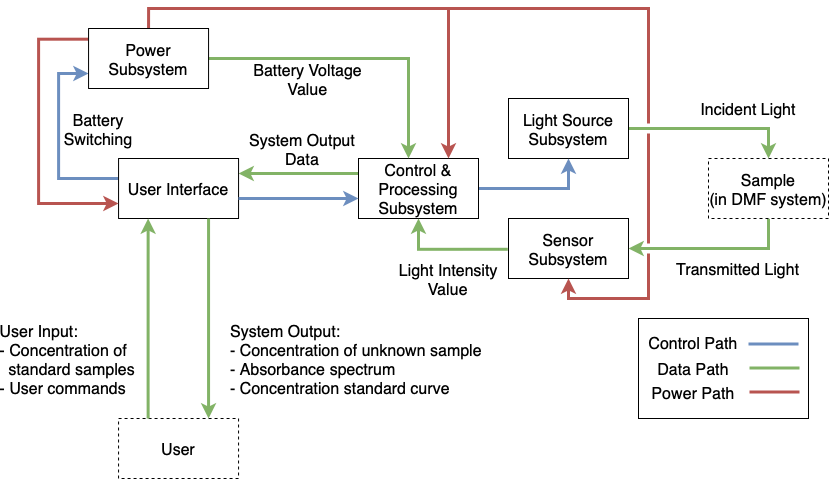
\includegraphics[scale=0.27]{system-dfd.png}}
    \caption{Level-1 Data Flow Diagram (DFD) of the system}
    \label{system-dfd}
    \end{figure}

    \begin{figure}[htbp]
    \centerline{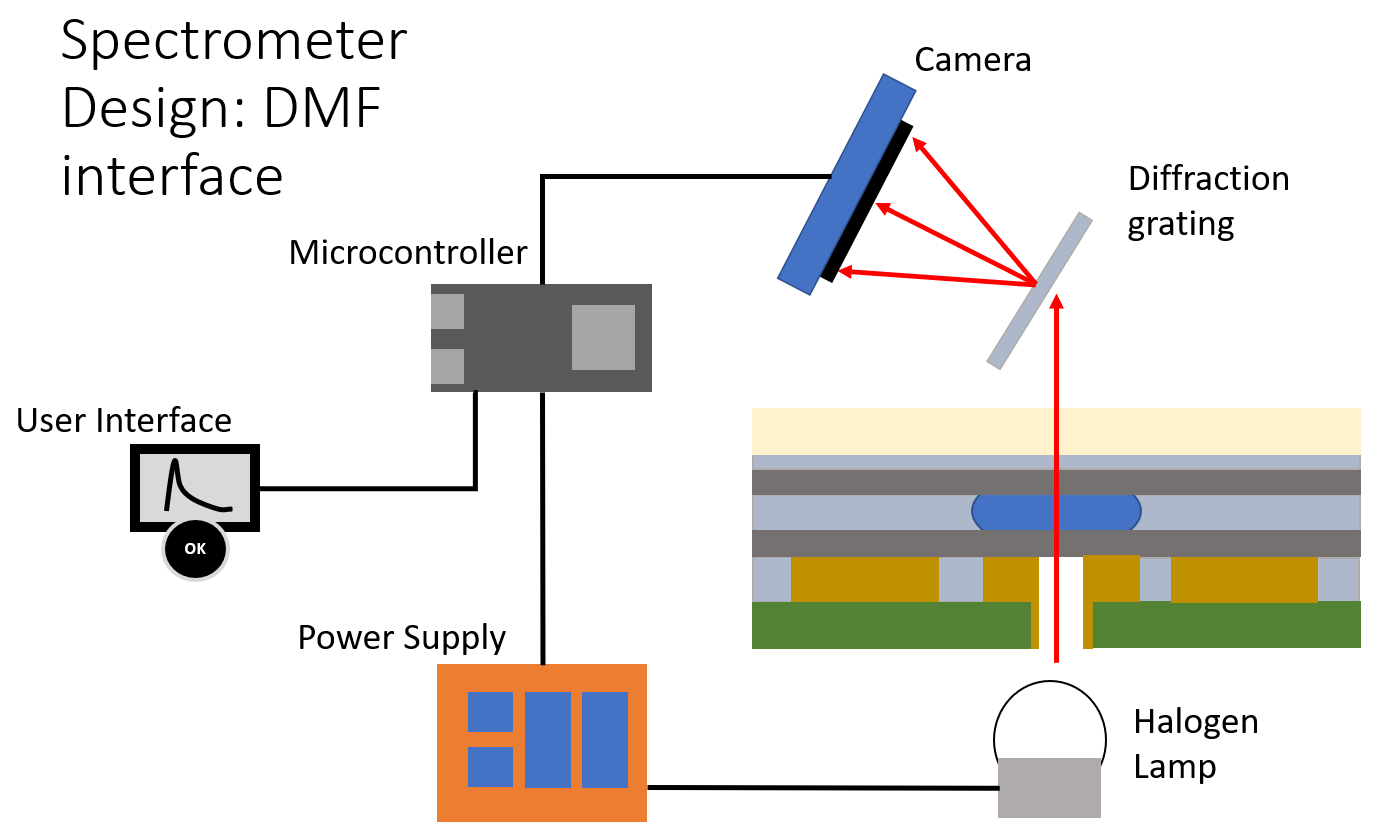
\includegraphics[scale=0.27]{dmf-hardware-scheme.png}}
    \caption{The main components of the proposed device}
    \label{dmf-hardware-scheme}
    \end{figure}

\subsection{Light Source Subsystem}
The light source subsystem functions to produce polychromatic light as the primary variable to be manipulated and measured by the instrument.
This subsystem includes 2 modules, namely switching circuits and light sources.
The process in this subsystem begins with receiving a control signal from the control subsystem to the switching circuit.
The switching circuit then flows the source voltage to the lamp so that it can be lit.
The polychromatic light source will illuminate and produce light with all UV-Vis frequencies within the specification.
This light is then passed on to the sample for a certain period.

\subsection{Light Sensor Subsystem}
The light sensor subsystem functions as a spectrometer that receives polychromatic light beam and outputs light intensities of discrete wavelengths in the form of digital data.
Polychromatic light beam enters the sensor subsystem through a hole and gets diffracted by a transmissive diffraction grating as to spatially separate light by its wavelengths.
The grating has a groove density of 1200 lines/mm, and the first order of diffraction is used to separate the visible spectrum.
The resulting ray is then recorded by a CMOS image sensor (Arducam MT9M001 Monochrome Camera Module).
Different pixel of the image sensor captures the intensity of different wavelengths ranging from 400 nanometer to 700 nanometer formatted into 10-bit unsigned integer.
The light sensor subsystem outputs, at maximum, 400 16-bit unsigned integer values, each value representing the light intensity of wavelengths in the visible spectrum range. 

\subsection{Control and Processing Subsystem}
The control and processing subsystem consists of control and data processing unit.
Other subsystems in the spectrophotometer are controlled by a ESP32-S3-DevkitC-1 microcontroller board (Espressif Systems, China)/
The task of the control unit is to execute the main workflow of the spectrophotometer by a FSM.
The control subsystem synchronizes other subsystems, such as the light source with the light sensor when measuring light intensities.
The processing of data signals for measurement processes and results is a responsibility of the data processing unit.
It converts the sensor's intensity data into an absorbance spectrum (spectrum mode) and performs linear regression to calculate the sample concentration according to the standard samples.

C++ programming was used to create the control subsystem program, and the PlatformIO IDE for Microsoft Visual Studio Code was used (VSCode).
The primary responsibility of the control unit is to execute the spectrophotometer's processes based on the designed Finite State Machine (FSM), as shown in Fig. \ref{fsm}.

    \begin{figure}[htbp]
    \centerline{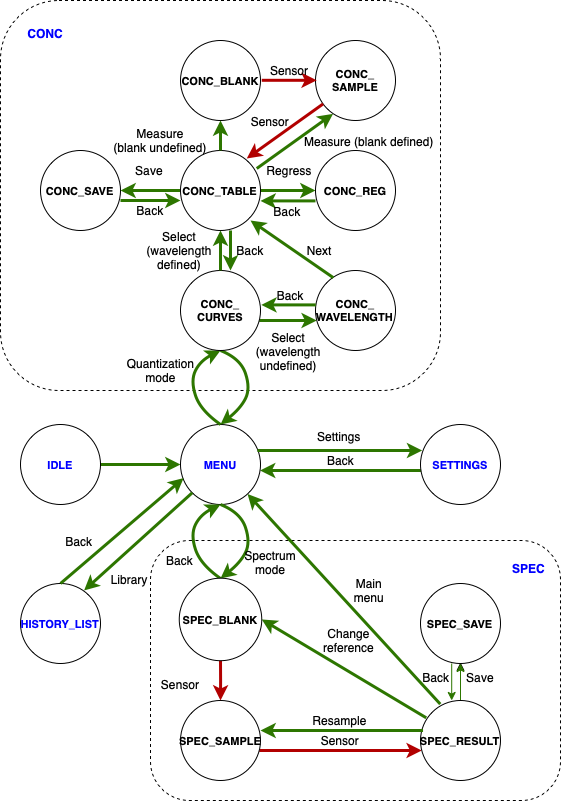
\includegraphics[scale=0.35]{fsm.png}}
    \caption{FSM diagram of the portable visible spectrophotometer}
    \label{fsm}
    \end{figure}

The absorbance \emph{A} of a particular sample is computed by the Equation (\ref{absorbance}).

    \begin{equation}
    A=-\log10{T}=\log{\frac{{I_{0}}{I}}}
    \label{absorbance}
    \end{equation}

Transmittance \emph{T} is the percentage of incident radiation that the sample transmits, \emph{I_{0}} denotes the intensity of polychromatic light entering the sample, and \emph{I} denotes the intensity of light leaving the sample;
Absorbance is directly proportional to the path length \emph{l} through the medium and the concentration \emph{c} of the absorbing substance for monochromatic radiation.
Beer-Lambert's law, expressed in Equation (\ref{beer-lambert}), serves as the basis for quantitative analyses using both atomic and molecular absorption measurements (\emph{\epsilon} is the molar attenuation coefficient)\cite{b4}.

    \begin{equation}
    A={\epsilon}{l}{c}
    \label{beer-lambert}
    \end{equation}

Beer-Lambert's law states that the concentration of a dilute solution is directly proportional to its absorbance value.
As a result, in the quantization mode, a linear regression is performed to obtain a slope-intercept form linear equation, as follows. 

    \begin{equation}
    A={m}{c}+{b}
    \label{linear-eq}
    \end{equation}

where m is the line's slope (gradient) and b is the constant representing the linear equation's y-intercept.

The measurement data are stored on an external SD card that is part of the data processing device.
The data for the absorbance spectrum and the calibration curves for the quantization mode are tabulated in a CSV-file format.
The interface between the micro-SD card and the control system is provided by a microSD click module (MikroElektronika, Serbia).
In order to store calibration values for absorbance measurement and quantization-mode calibration curves, the microcontroller also utilizes its non-volatile memory storage (NVS).

\subsection{User Interface Subsystem}
The user interface subsystem plays a role in connecting the system and the users.
This can be done by interpreting the commands given by users through the input interface devices and process it into control signals that will be sent to the control subsystem.
The subsystem also has a function to display measurement data which include sample concentration values, sample absorbance spectrum, regression curves, menus, and settings.
Fig. \ref{ui-dfd} shows the data flow diagram of the user interface subsystem.

Four push buttons and a power switch are used as the input interface devices.
For the display, a 3.5-inch non-touchscreen TFT LCD with ILI9488 driver is used.
The configuration of buttons and non-touchscreen LCD is chosen because it fits the users who use the spectrophotometer using laboratory gloves.

    \begin{figure}[htbp]
    \centerline{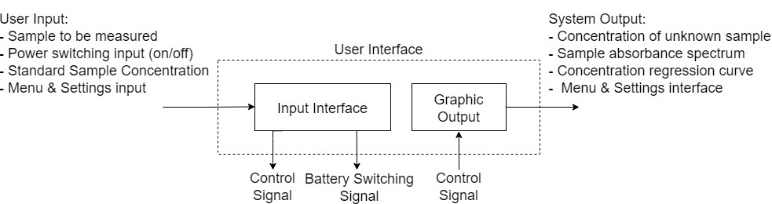
\includegraphics[scale=0.43]{ui-dfd.png}}
    \caption{DFD of the user interface subsystem}
    \label{ui-dfd}
    \end{figure}


\subsection{Power Subsystem}
The power subsystem enables the system to be activated by supplying power from the battery to the entire electrical circuit. The battery can be recharged easily whenever the battery voltage is insufficient. The power subsystem also provides information about the battery voltage value to be displayed to the user. 

    \begin{figure}[htbp]
    \centerline{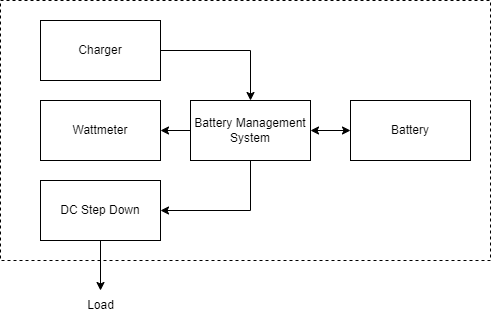
\includegraphics[scale=0.5]{power-dfd.png}}
    \caption{DFD of the power subsystem}
    \label{power-dfd}
    \end{figure}

The power subsystem is activated when the user presses the power button for the first time—allowing the power to flow to the microcontroller. The microcontroller will supply power to certain sub-blocks according to user input by adjusting the whether the battery voltage is sufficient based on a specified threshold. If the battery voltage value is below the threshold or the user presses the power button again, the power supply to the entire circuit will be cut off, and the system will be disabled.

\subsection{Hardware Assembly}
Using Autodesk Fusion 360 software, the body and individual parts of the portable visible spectrophotometer were created and 3D printed.
The primary body, the optical light path, and the lamp holder were all 3D printed components.
Fig.~\ref{hardware} displays internal components of the device.
A polylactic acid (PLA) filament in black was used due to the need of low light reflectance.
Electronic parts like printed circuit boards (PCBs) and optical parts were placed inside the main body.

    \begin{figure}[htbp]
    \centerline{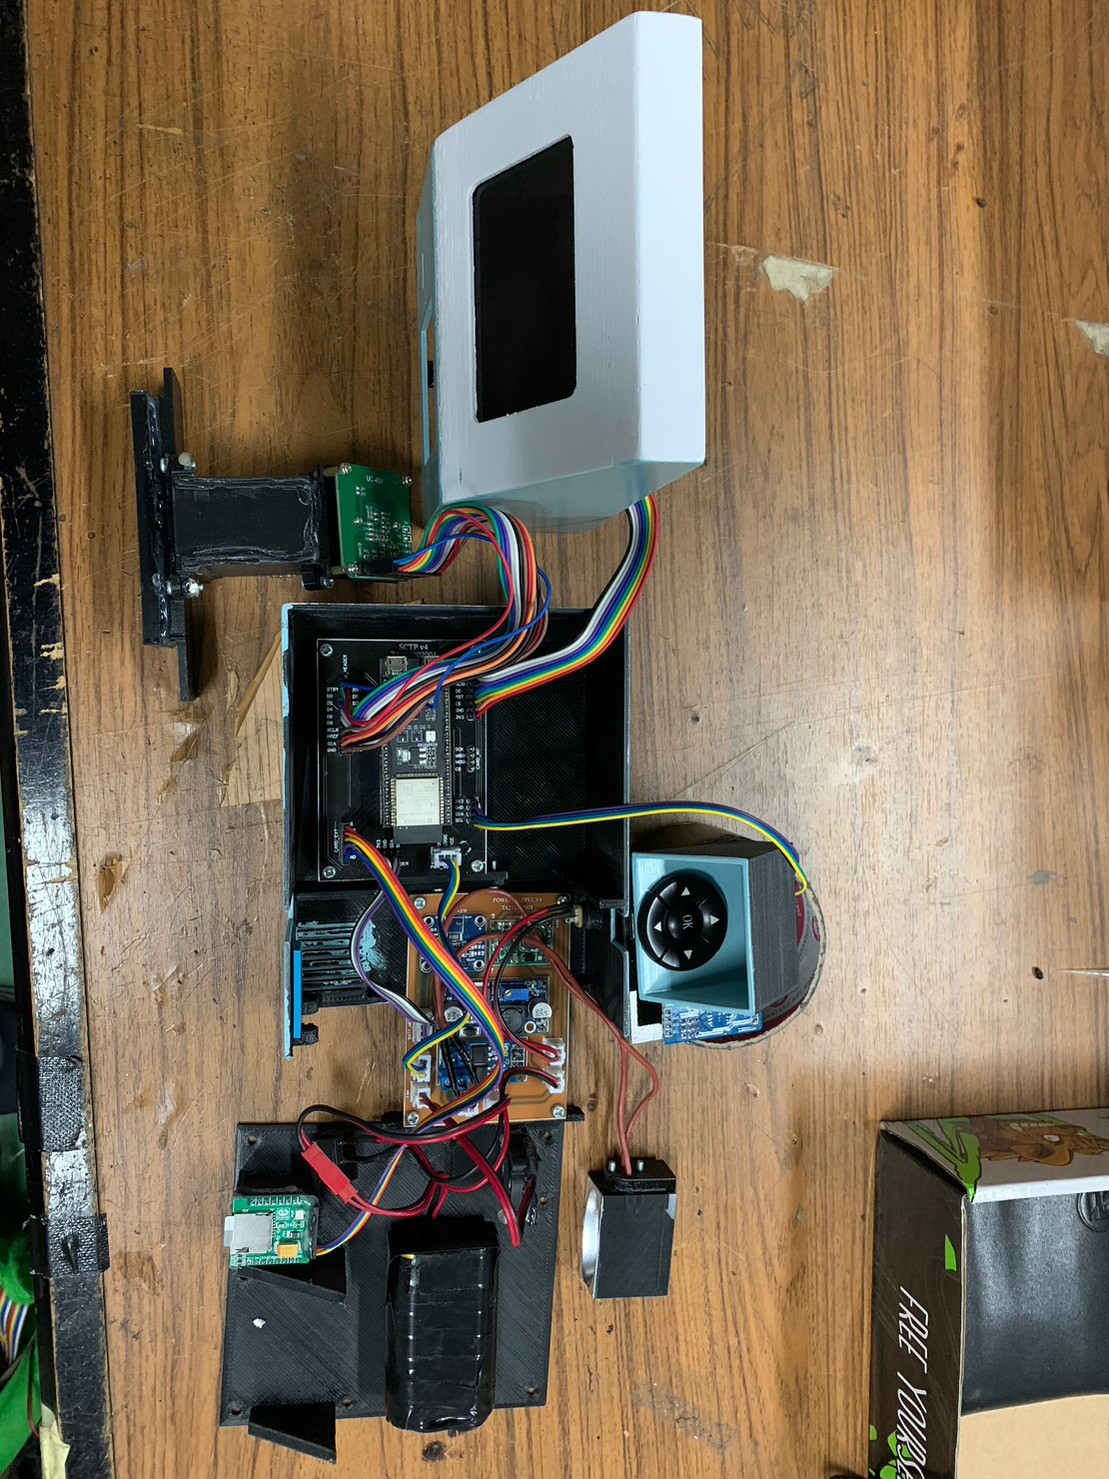
\includegraphics[scale=0.15]{hardware-2.jpg}}
    \caption{Overview of the device's internal components}
    \label{hardware}
    \end{figure}

\section{Results and Discussion}
\subsection{Accuracy}
A glucose assay kit (Glucose (GO) Assay Kit, Sigma-Aldrich) was used to colorize glucose sample of 40 {\textmu}g/ml and 60 {\textmu}g/ml concentration.
The resulting liquid was then dropped between two microscope slides spaced 1 mm apart to mimic the light path of the DMF cartridge.

Fig.~\ref{glucose_result} shows the measurement results of the glucose experiment with baseline correction using linear regression.
Manual baseline correction was found necessary because of a voltage fluctuation found between blank measurement and sample measurement.
Peak absorbance were measured 0.155 at 519 nm for 40 {\textmu}g/ml and 0.079 at 526 nm for 60 {\textmu}g/ml.
Absorbance for the 40 {\textmu}g/ml sample turned out higher than the 60 {\textmu}g/ml sample.
This result does not fit the absorbance-concentration relation of the Beer-Lambert law.
It was also observed that the 40 {\textmu}g/ml sample appeared darker for the naked eye.
Thus, a retest of the chemical reactions was due.

    \begin{figure}[htbp]
    \centerline{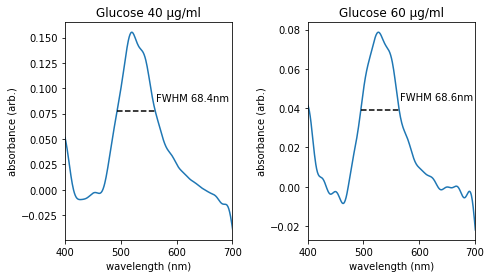
\includegraphics[scale=0.5]{glucose-res.png}}
    \caption{Glucose absorbance spectrum measurement result, baseline corrected}
    \label{glucose_result}
    \end{figure}

Aside from glucose, we have tested the spectrophotometer with food dye measurements.
Blue, red, and yellow food dyes were mixed with water.
The volume percentage used were 0.033\%, 0.040\%, 0.050\%, 0.067\%, and 0.100\%.
% The samples were then dropped to the DMF cartridge as shown in Fig. \ref{dye_setup}.
The cartridge consisted of a DMF cartridge PCB, a layer of stretched parafilm, and a layer of silicon oil underneath the droplet;
a layer of silicon oil, a layer of stretched parafilm, and a layer of ITO above the droplet. 

\begin{figure}[htbp]
    \centerline{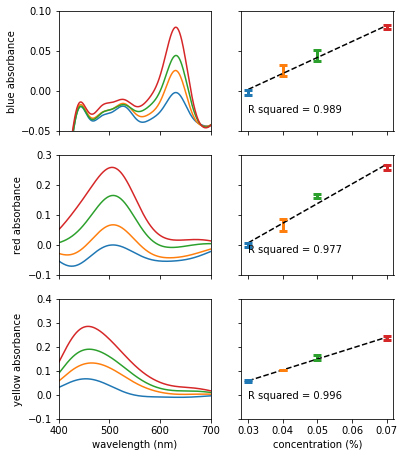
\includegraphics[scale=0.6]{dye-res.png}}

    \caption{Dye measurement results}
    \label{dye_res}
    \end{figure}

Measurements of the food dye samples were regressed as shown in Fig. \ref{dye_res} to create standard curves.
The wavelengths of which the absorbance were measured were the peak absorbances of each dye.
An upward trend was found in accordance to the Beer-Lambert law.
The coefficient of determination measured decreased as the wavelength decreased.
Accuracy was expected to decrease as wavelength decreases due to weakening lamp emission and camera spectrum response at low wavelengths.

\subsection{Repeatability}
\subsection{Wavelength Range}
\subsection{Resolution}
Resolution testing is carried out by calculating the resolution of the measurement results stored on an external SD card in the form of a CSV file.
The number of pixels needed for the absorbance spectrum measurement, which is obtained from the calibration results, was 297.
The absorbance measurement results are stored on an external SD card with a resolution that can be calculated using Equation (\ref{resolution}).

    \begin{equation}
    resolution=\frac{\lambda_{max} - \lambda_{min}}{n_{pixels}}=\frac{(700 - 400)nm}{393}\approx0.77nm
    \label{resolution}
    \end{equation}

\subsection{Device and DMF Cartridge Distance}

\subsection{Weight and Size}
Weight measurement is done by placing the product on a digital scale.
The product's weight is 0.832 kilograms.

% \begin{figure}[htbp]
%     \centerline{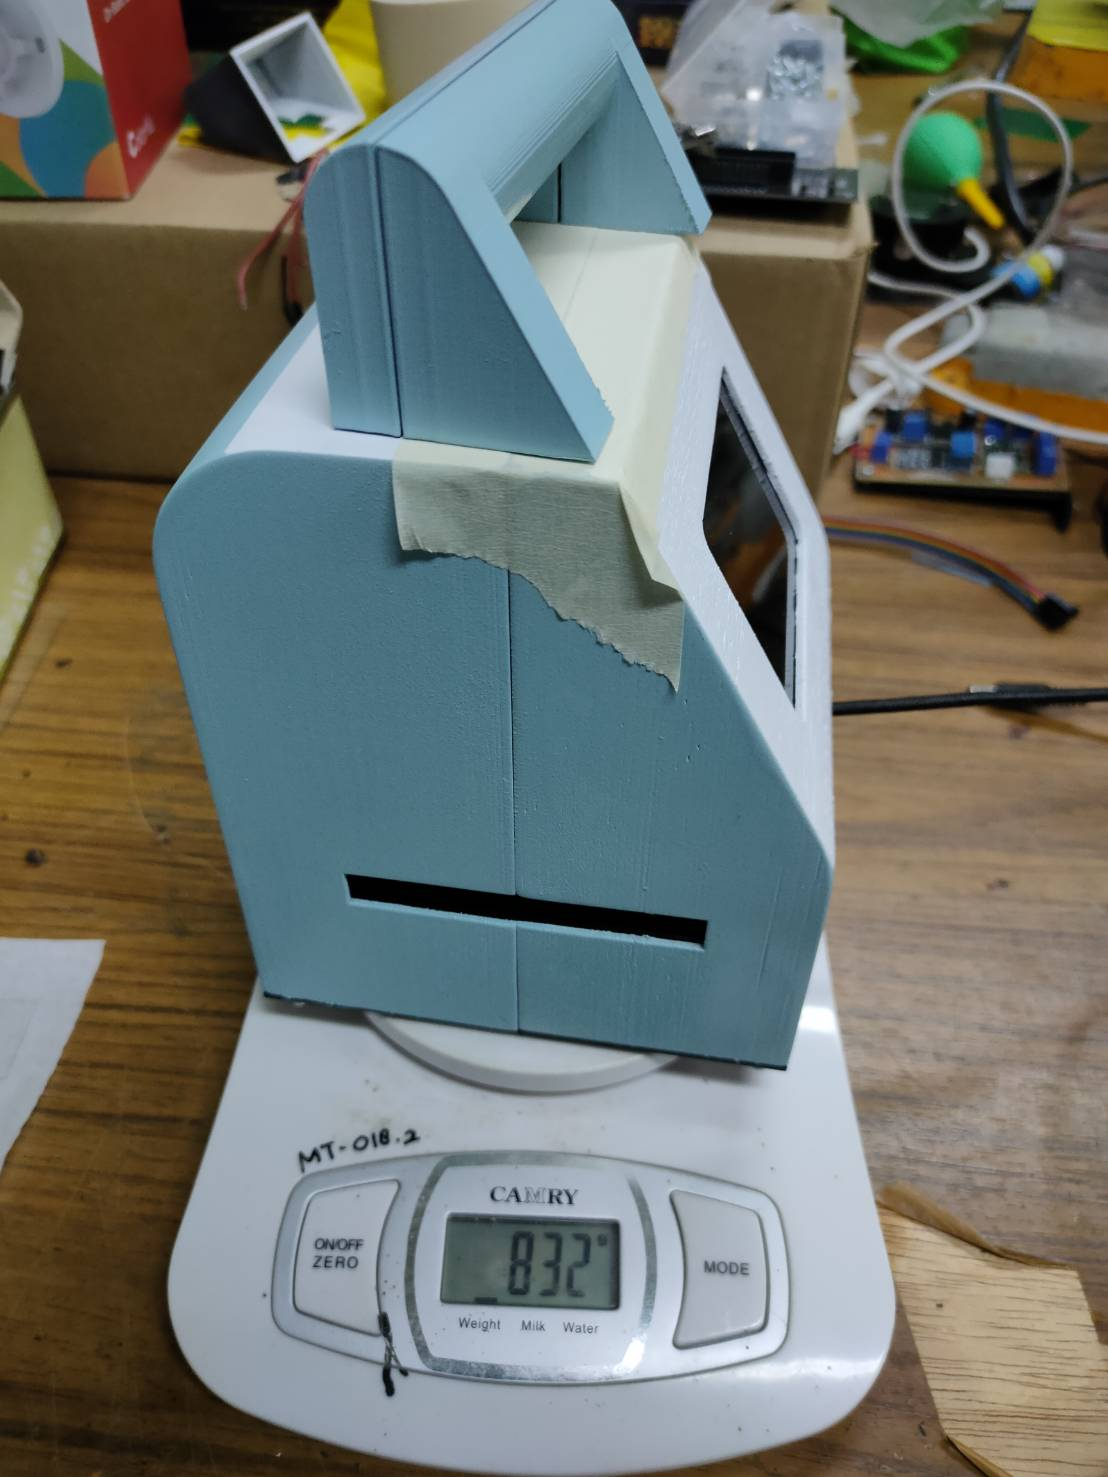
\includegraphics[scale=0.12]{SCTP_weight.jpg}}
%     \caption{Device's weight measurement}
%     \label{device_weight}
%     \end{figure}

The dimension produced are 120 mm x 131 x 207 mm, as shown in Fig. \ref{device_dimensions}
Product dimensions are affected by the number of components used in the system and the optical configuration used. 
The sensor's location, diffraction grating, and light source mainly influence the product's height. 
The battery has a size of 70 x 42 x 21 mm, which significantly affects the determination of the minimum area of the product base.
In addition, the button component with a diagonal position uses a large enough area but leaves quite a lot of remaining space.

\begin{figure}[htbp]
    \centerline{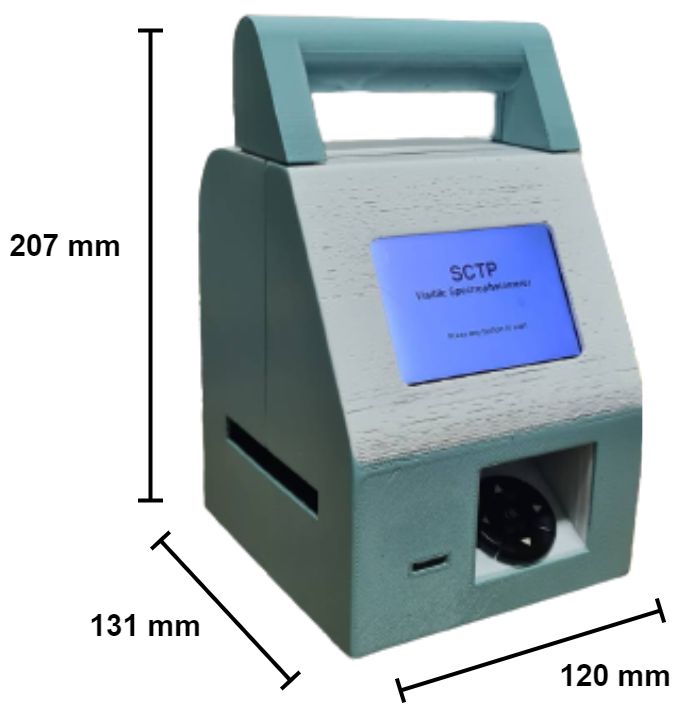
\includegraphics[scale=0.25]{SCTP_size.png}}
    \caption{Device's dimensions}
    \label{device_dimensions}
    \end{figure}

\subsection{User Interface}
The first page of the spectrum-mode measurement instructs the user to insert the blank reference sample into the DMF system.
The sample input page, which resembles the blank input page, will be on the next page.
A result page with the peak wavelength and absorbance results will show up after the other subsystems have finished measuring absorbance.
The user has the option to save the result, return to the main menu, or view the entire spectrum of the absorbance measurement.
Fig. \ref{lcd-spectrum} illustrates how the spectrum page of the absorbance measurement is shown.

    \begin{figure}[htbp]
    \centerline{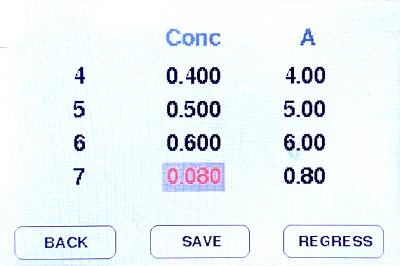
\includegraphics[scale=0.6]{lcd-spectrum.png}}
    \caption{The display of the spectrum page of a spectrum-mode measurement}
    \label{lcd-spectrum}
    \end{figure}

Quantization-mode measurement starts with a page that displays the list of saved curves.
Users have the option of using, removing, or adding new curves.
The user will get a table page if they select an existing curve.
The table consists of concentration and absorbance values of standard samples, as shown in Fig. \ref{lcd-table}.
By moving the pointer to the desired absorbance (A) cell and clicking the OK physical button, an absorbance measurement for each concentration value should be made.
The user will be directed to the blank and sample input page.
The user should click the REGRESS button to calculate the concentration of the unknown sample and view the standard curve plot.

    \begin{figure}[htbp]
    \centerline{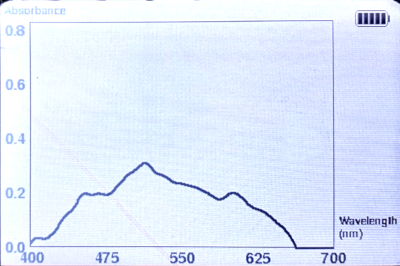
\includegraphics[scale=0.6]{lcd-table.png}}
    \caption{The display of the table page of a quantization-mode curve}
    \label{lcd-table}
    \end{figure}

\section{Conclusions}
To support the study of spectrophotometry analysis in DMF platform, we describe the assembly of a portable spectrophotometer that can be integrated with a particular DMF system.
The portability makes on-the-go research processes easier.
Data acquisition, storage, and user experience is made simpler by our developed portable visible spectrophotometer and a user-friendly interface.
Measurement's accuracy of red, yellow, and blue food dyes and its repeatability demonstrated good performances in experimental validation versus commercial spectrophotometer (Evolution 220).
The colorimetric glucose assay (maximum of absorbance at 540 nm) measurements were comparable but quite inferior; these issues could be resolved by retesting the colorimetric reactions more thoroughly.
Future work will focus on designing a better voltage regulation and heat insulation for the lamp, as well as designing reducing movable parts from the light path configuration.

\section*{References}


\begin{thebibliography}{00}
\bibitem{b1} H. V. Tran et al., “Silver nanoparticles-decorated reduced graphene oxide: A novel peroxidase-like activity nanomaterial for development of a colorimetric glucose biosensor,” Arabian Journal of Chemistry, vol. 13, no. 7, pp. 6084–6091, Jul. 2020, doi: 10.1016/j.arabjc.2020.05.008.
\bibitem{b2} Z. Gu, M. L. Wu, B. Y. Yan, H. F. Wang, and C. Kong, “Integrated Digital Microfluidic Platform for Colorimetric Sensing of Nitrite,” ACS Omega, vol. 5, no. 19, pp. 11196–11201, May 2020, doi: 10.1021/acsomega.0c01274.
\bibitem{b3} S. Huang and R. B. Fair, “Quantitative measurements of inorganic analytes on a digital microfluidics platform,” SN Applied Sciences, vol. 1, no. 12, Dec. 2019, doi: 10.1007/s42452-019-1693-8.
\bibitem{b4} D. A. Skoog, F. J. Holler, and S. R. Crouch, Principles of Instrumental Analysis, 7th ed. Cengage Learning, 2016.
\end{thebibliography}

\end{document}